\documentclass{beamer}
\usepackage{graphicx} % Required for inserting images
\usetheme{Madrid}
\usepackage{tikz}
\usepackage{xcolor}



\usepackage{xcolor}
\definecolor{DoctorWhoBlue}{RGB}{16, 35, 97}  % TARDIS Blue color



%Customising my arrows 
\tikzstyle{box} = [rectangle, rounded corners, minimum width=3cm, minimum height=1cm,text centered, draw=black, fill=blue!10]
\tikzstyle{arrow} = [thick,->,>=stealth]

\title{Election Outcomes and Democratic Trust}
\author{Tie Ma \& Robert Ta-Chuan Yu}
\date{March 03, 2025}

\begin{document}
\maketitle

\begin{frame}
\frametitle{Research Question \& Motivation}
\vspace{-1.5cm}
\begin{block}
{Question} How does the outcome of the 2021 Canadian federal election influence voters' trust and satisfaction with democracy, particularly in relation to whether their preferred party secured electoral victory?
\end{block}
\bigskip{}

\textbf{Motivation}
\begin{itemize}
    \item The instability of the U.S. democratic system caused by President Trump shows that democracy is not as indestructible as people expect.
    \item Although statistical methods are commonly used in political science research but limit to simplified model. 
\end{itemize}
\end{frame}

%%%%%%%%%
%%%%%%%%%
\begin{frame}
    \frametitle{Canadian Politics}
    \begin{itemize}
        \item Constitutional democracy.
        \item First-Past-the-Post electoral system.
        \item 338 ridings, with 170 seats needed to win a majority government.
        \item Five major parties: Liberal, Conservative, NDP, Bloc Québécois, and Green Party.
    \end{itemize}
\end{frame}



%%%%%%%%%
\begin{frame}
    \frametitle{2021 Federal Election Results}
    \centering
    \includegraphics[width=0.8\textwidth]{Canada_Election_2021_Results_Map.pdf} % Adjust width as needed
\end{frame}
%%%%%



%%%%%%%%%%%%%%%%%%%%%%%%%%%%%%%%%%%%%%%%%%%%%%%%%%%%%%%%%%%%%%%%%%%%%%%%%%%%%%%%%%%%%%%%


\usetikzlibrary{shapes.geometric, arrows}

\tikzstyle{box} = [rectangle, rounded corners, minimum width=3cm, minimum height=1cm, text centered, draw=black, fill=blue!10]
\tikzstyle{arrow} = [thick,->,>=stealth]



\begin{frame}
\frametitle{Motivation in Theory}
\begin{center}
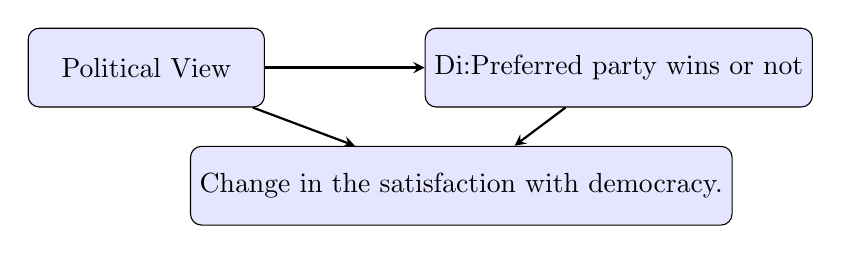
\begin{tikzpicture}

% Nodes
\node (PV) [box] at (-2,1.5) {Political View};  % Top-left
\node (TV) [box] at (4,1.5) {Di:Preferred party wins or not}; % Top-right
\node (change) [box] at (2,0) {Change in the satisfaction with democracy.}; % Bottom-center

% Arrows
\draw [arrow] (PV) -- (change);
\draw [arrow] (TV) -- (change);
\draw [arrow] (PV) -- (TV);

\end{tikzpicture}
\end{center}
\end{frame}

%%%%%%%%%%%%%%%%%%%%%%%%%%%%%%%%%%%%%%%%%%%%%%%%%%%%%%%%%%%%%%%%%%%%%%%%%%%%%%%%%%%%%%%%%%%%%
\begin{frame}
    \frametitle{Hypotheses}
    \begin{itemize}
        \item \textbf{Electoral Winner-Loser Hypothesis:} Voters who supported the winning party in an election tend to express greater satisfaction democracy compared to those who supported a losing party.
        \item []
        \item \textbf{Political View Alignment Hypothesis:} Voters whose political views align with the winning party in an election tend to be more satisfied with democracy than those whose views do not.
    \end{itemize}
\end{frame}
%%%%%%%%%%%%%%%%%%%%%%%%%%%%%%%%%%%%%%%%%%%%%%%%%%%%%%%%%%%%%%%%%%%%%%%%%%%%%%%%%%%%%%%%%%%%%



%%%%%%%%%%%%%%%%%%%%%%%%%%%%%%%%%%%%%%%%%%%%%%%%%%%%%%%%%%%%%%%%%%%%%%%%%%%%%%%%%%%%%%%%%%%%%



\begin{frame}
    \frametitle{Data Availability}
    \begin{itemize}
        \item Canadian Election Study 2021 (CES)
        \item Surveyed over 10,000 Canadians both before and after the election.
        \item Comprises a total of 1,062 variables.
        \item The survey design aimed to mirror the geographic distribution of Canada.
        \item Pre-election survey conducted from August 17, 2021 to September 19, 2021.
        \item Post-election survey conducted from September 23, 2021 to October 4, 2021.
    \end{itemize}
\end{frame}


%%%%%%%%%%%%%%%%%%%%%%%%%%%%%%%%%%%%%%%%%%%%%%%%%%%%%%%%%%%%%%%%%%%%%%%%%%%%%%%%%%%%%%%%%%%%%




%%%%%%%%%%%%%%%%%%%%%%%%%%%%%%%%%%%%%%%%%%%%%%%%%%%%%%%%%%%%%%%%%%%%%%%%%%%%%%%%%%%%%%%%%%%%%
\begin{frame}
    \frametitle{Compare Gender and Party Distribution}
    \begin{center}
        \begin{minipage}{0.48\textwidth} % Gender Distribution (Left)
            \centering
            \textbf{Gender Distribution} \\ % 标题
            \vspace{0.3cm} % 调整标题和图片间距
            \raisebox{-0.5cm}{ % 解决垂直对齐问题
                \includegraphics[width=0.9\textwidth, height=5cm, keepaspectratio]{Gender Distribution in CES 2021.pdf}
            }
        \end{minipage}
        \hfill
        \begin{minipage}{0.48\textwidth} % Party Distribution (Right)
            \centering
            \textbf{Party Distribution} \\ % 标题
            \vspace{-0.3cm} % 调整标题和图片间距
            \raisebox{-0.5cm}{ % 解决垂直对齐问题
                \includegraphics[width=0.9\textwidth, height=5cm, keepaspectratio]{Party Distribution in CES 2021.pdf}
            }
        \end{minipage}
    \end{center}
\end{frame}
%%%%%%%%%%%%%%%%%%%%%%%%%%%%%%%%%%%%%%%%%%%%%%%%%%%%%%%%%%%%%%%%%%%%%%%%%%%%%%%%%%%%%%%%%%%%%





%%%%%%%%%%%%%%%%%%%%%%%%%%%%%%%%%%%%%%%%%%%%%%%%%%%%%%%%%%%%%%%%%%%%%%%%%%%%%%%%%%%%%%%%%%%%%
\begin{frame}
    \frametitle{Liberal vs. NDP Satisfaction Comparison}
    \begin{center}
        \begin{minipage}{0.48\textwidth} % Liberal on the left
            \centering
            \textbf{\textcolor{red}{Liberal}} \\ % Liberal in Red
            \includegraphics[width=\textwidth]{Pre-election vs. Post-election Satisfaction for Liberal.pdf}
        \end{minipage}
        \hfill
        \begin{minipage}{0.48\textwidth} % NDP on the right
            \centering
            \textbf{\textcolor{orange}{NDP}} \\ % NDP in Orange
            \includegraphics[width=\textwidth]{Pre-election vs. Post-election Satisfaction for NDP.pdf}
        \end{minipage}
    \end{center}
\end{frame}
%%%%%%%%%%%%%%%%%%%%%%%%%%%%%%%%%%%%%%%%%%%%%%%%%%%%%%%%%%%%%%%%%%%%%%%%%%%%%%%%%%%%%%%%%%%%%




%%%%%%%%%%%%%%%%%%%%%%%%%%%%%%%%%%%%%%%%%%%%%%%%%%%%%%%%%%%%%%%%%%%%%%%%%%%%%%%%%%%%%%%%%%%%%
\begin{frame}
    \frametitle{Liberal vs. Conservative Satisfaction Comparison}
    \begin{center}
        \begin{minipage}{0.48\textwidth} % Liberal on the left
            \centering
            \textbf{\textcolor{red}{Liberal}} \\ % Liberal in Red
            \includegraphics[width=\textwidth]{Pre-election vs. Post-election Satisfaction for Liberal.pdf}
        \end{minipage}
        \hfill
        \begin{minipage}{0.48\textwidth} % NDP on the right
            \centering
            \textbf{\textcolor{blue}{Conservative}} \\ % NDP in Orange
            \includegraphics[width=\textwidth]{Pre-election vs. Post-election Satisfaction for Conservative.pdf}
        \end{minipage}
    \end{center}
\end{frame}
%%%%%%%%%%%%%%%%%%%%%%%%%%%%%%%%%%%%%%%%%%%%%%%%%%%%%%%%%%%%%%%%%%%%%%%%%%%%%%%%%%%%%%%%%%%%%






%%%%%%%%%%%%%%%%%%%%%%%%%%%%%%%%%%%%%%%%%%%%%%%%%%%%%%%%%%%%%%%%%%%%%%%%%%%%%%%%%%%%%%%%%%%%%
\begin{frame}
    \frametitle{Question?} % Slide title
    \begin{center}
        \vspace{1.5cm} % Adds some space from the top
        {\Huge Any Questions?} % Makes the text large
        \vspace{1.5cm} % Adds space below the text
    \end{center}
\end{frame}
%%%%%%%%%%%%%%%%%%%%%%%%%%%%%%%%%%%%%%%%%%%%%%%%%%%%%%%%%%%%%%%%%%%%%%%%%%%%%%%%%%%%%%%%%%%%%

%%%%%%%%%%%%%%%%%%%%%%%%%%%%%%%%%%%%%%%%%%%%%%%%%%%%%%%%%%%%%%%%%%%%%%%%%%%%%%%%%%%%%%%%%%%%%
\begin{frame}
    \frametitle{References} % Slide title

    \begin{flushleft}
        \textbf{Elections Canada}, Official Voting Results - 45th General Election Results\\
        \url{https://www.elections.ca/res/rep/off/ovr2021app/home.html}
        
        \vspace{1.0cm} % Adds space below the text

        \textbf{Stephenson, Laura B., Allison Harell, Daniel Rubenson, and Peter John Loewen.}\\
        \textit{The 2021 Canadian Election Study.}
    \end{flushleft}

\end{frame}
%%%%%%%%%%%%%%%%%%%%%%%%%%%%%%%%%%%%%%%%%%%%%%%%%%%%%%%%%%%%%%%%%%%%%%%%%%%%%%%%%%%%%%%%%%%%%


%%%%%%%%%%%%%%%%%%%%%%%%%%%%%%%%%%%%%%%%%%%%%%%%%%%%%%%%%%%%%%%%%%%%%%%%%%%%%%%%%%%%%%%%%%%%%
\begin{frame}
    \frametitle{Pre-election vs. Post-election Satisfaction for Liberal Party}
    \begin{center}
        \includegraphics[scale=0.3]{Pre-election vs. Post-election Satisfaction for Liberal.pdf}
    \end{center}
\end{frame}
%%%%%%%%%%%%%%%%%%%%%%%%%%%%%%%%%%%%%%%%%%%%%%%%%%%%%%%%%%%%%%%%%%%%%%%%%%%%%%%%%%%%%%%%%%%%%


%%%%%%%%%%%%%%%%%%%%%%%%%%%%%%%%%%%%%%%%%%%%%%%%%%%%%%%%%%%%%%%%%%%%%%%%%%%%%%%%%%%%%%%%%%%%%

\begin{frame}
    \frametitle{Pre-election vs. Post-election Satisfaction for Conservative Party}
    \begin{center}
        \includegraphics[scale=0.3]{Pre-election vs. Post-election Satisfaction for Conservative.pdf}
    \end{center}
\end{frame}
%%%%%%%%%%%%%%%%%%%%%%%%%%%%%%%%%%%%%%%%%%%%%%%%%%%%%%%%%%%%%%%%%%%%%%%%%%%%%%%%%%%%%%%%%%%%%




%%%%%%%%%%%%%%%%%%%%%%%%%%%%%%%%%%%%%%%%%%%%%%%%%%%%%%%%%%%%%%%%%%%%%%%%%%%%%%%%%%%%%%%%%%%%%

\begin{frame}
    \frametitle{Pre-election vs. Post-election Satisfaction for Bloc Party}
    \begin{center}
        \includegraphics[scale=0.3]{Pre-election vs. Post-election Satisfaction for Block.pdf}
    \end{center}
\end{frame}
%%%%%%%%%%%%%%%%%%%%%%%%%%%%%%%%%%%%%%%%%%%%%%%%%%%%%%%%%%%%%%%%%%%%%%%%%%%%%%%%%%%%%%%%%%%%%

%%%%%%%%%%%%%%%%%%%%%%%%%%%%%%%%%%%%%%%%%%%%%%%%%%%%%%%%%%%%%%%%%%%%%%%%%%%%%%%%%%%%%%%%%%%%%


\begin{frame}
    \frametitle{Pre-election vs. Post-election Satisfaction for NDP}
    \begin{center}
        \includegraphics[scale=0.3]{Pre-election vs. Post-election Satisfaction for NDP.pdf}
    \end{center}
\end{frame}
%%%%%%%%%%%%%%%%%%%%%%%%%%%%%%%%%%%%%%%%%%%%%%%%%%%%%%%%%%%%%%%%%%%%%%%%%%%%%%%%%%%%%%%%%%%%%

%%%%%%%%%%%%%%%%%%%%%%%%%%%%%%%%%%%%%%%%%%%%%%%%%%%%%%%%%%%%%%%%%%%%%%%%%%%%%%%%%%%%%%%%%%%%%

\begin{frame}
    \frametitle{Pre-election vs. Post-election Satisfaction for Green Party}
    \begin{center}
        \includegraphics[scale=0.3]{Pre-election vs. Post-election Satisfaction for green.pdf}
    \end{center}
\end{frame}
%%%%%%%%%%%%%%%%%%%%%%%%%%%%%%%%%%%%%%%%%%%%%%%%%%%%%%%%%%%%%%%%%%%%%%%%%%%%%%%%%%%%%%%%%%%%%





%%%%%%%%%%%%%%%%%%%%%%%%%%%%%%%%%%%%%%%%%%%%%%%%%%%%%%%%%%%%%%%%%%%%%%%%%%%%%%%%%%%%%%%%%%%%%





\end{document}


